\section{EXPERIMENTS}
\label{sec:experiments}

\subsection{Setup}
\label{sec:exp_setup}

We evaluate HE-IFD on two image classification datasets (CIFAR-10~\cite{krizhevsky2009learning} and FashionMNIST~\cite{xiao2017fashion}) with two model families (ResNet-18 and SimpleCNN), and extend the evaluation to pre-trained Vision Transformers (ViT-B/32). All accuracy experiments run as plaintext simulations of the encrypted protocol to expedite the evaluation: we execute the exact same forward and backward passes, loss functions, and weight updates that the CKKS-encrypted server would perform, and validate numerical equivalence against TenSEAL-based encrypted operations in Section~\ref{sec:ckks_validation}.

\textbf{Data partitioning.} Client data is split using a Dirichlet distribution with concentration parameter $\alpha$, where a smaller $\alpha$ produces more heterogeneous partitions. We use $\alpha \in \{0.1, 1.0\}$ (extremely heterogeneous and heterogeneous) across $N \in \{1, 2, 4, 8, 16, 32\}$ clients.

\textbf{ResNet-18.} Each client trains a ResNet-18 teacher (11.2M parameters) for 200 epochs. The server distils into a PolyResNet-18 student with polynomial activations and per-channel affine scaling. Phase 2 trains each block independently on encrypted teacher features (80 epochs per block), then refines the cascade sequentially with bootstrapping to close the train-inference distribution gap. Each client contributes only 5000 samples (10\% of CIFAR-10's 50,000 training images). This is a deliberate experiment choice, as intermediate feature distillation is data-efficient because teacher features provide direct per-block supervision, and the server trains on pooled features from all clients. Using a small fraction of each client's data keeps the upload volume manageable while achieving strong accuracy.

\textbf{SimpleCNN.} We train SimpleCNN teachers (0.3M parameters, 4 conv layers) and distil into an HE-compatible polynomial student. %The pattern matches ResNet-18 across all settings.

\textbf{Vision Transformer.} We fine-tune pre-trained ViT-B/32 (ImageNet-1K, 88M parameters) on CIFAR-10 and FashionMNIST, replacing GELU with PolyGELU (degree-4) and LayerNorm with AffineNorm. %Oracle reaches 92\% on CIFAR-10 and 91\% on FashionMNIST. The same degradation pattern holds.

\begin{figure}[t]
\centering

\includegraphics[width=0.45\textwidth]{figures/fig_main_resnet18.pdf}
\caption{HE-IFD accuracy on CIFAR-10 (top) and FashionMNIST (bottom) with ResNet-18 teachers and PolyResNet-18 student. The two plaintext reference lines are the centralised Oracle (dashed gray, upper bound trained on all pooled data with no privacy protection) and the mean individual teacher accuracy at each setting (solid gray, the natural local-only floor each client could achieve without collaboration). HE-IFD (orange) approaches the Oracle at small $N$ and consistently outperforms the mean teacher across all settings.}
\label{fig:main_resnet18}
\end{figure}

\textbf{Reference points.} We anchor every accuracy curve in this section to two plaintext references that bracket the achievable range without our protocol:
\begin{itemize}[nosep]
    \item \textbf{Oracle}: a standard ResNet-18 trained on all pooled data in plaintext, with no privacy protection. This is the centralised upper bound on accuracy and the strongest possible baseline a non-private system could achieve.
    \item \textbf{Mean individual teacher}: the unweighted average accuracy of the $N$ local teacher models, each evaluated on the global test set after being trained only on its own private partition. This is the strongest accuracy that any client could obtain on its own without collaboration, and it is the relevant comparator for assessing whether participating in the protocol is worthwhile.
\end{itemize}
We do not include a separate plaintext-KL distillation baseline: the question this paper addresses is not how polynomial activations compare with ReLU under standard distillation (a centralised question, already studied in~\cite{baruch2022methodology, agamennone2025polynomial, alhossain2025training}), but whether a one-shot encrypted federated protocol can recover an accuracy that lies between the local-only mean teacher and the centralised Oracle.

In the rest of this section, \textbf{HE-IFD} refers to our method. For ResNet-18 experiments the student is PolyResNet-18, for SimpleCNN experiments, the student is HEStudentCNN, and for ViT experiments, the student is a ViT-B/32 with GELU replaced by PolyGELU and LayerNorm replaced by AffineNorm (Section~\ref{sec:arch_transformer}).

\subsection{Accuracy Results}
\label{sec:main_results}

Figure~\ref{fig:main_resnet18} shows accuracy across all settings on CIFAR-10 and FashionMNIST datasets. We summarize the key takeaways below: 

\textbf{HE-IFD consistently exceeds the mean teacher.} Across all settings with $\alpha \leq 1.0$, the encrypted student outperforms the average individual teacher by 10--20 percentage points. The student aggregates complementary knowledge from heterogeneous specialists into a single model that no individual client could construct from its own data alone.

% \textbf{HE-IFD approaches Oracle-level performance at low $N$.} On CIFAR-10, HE-IFD reaches 79.2\% at $N{=}1$ and $\sim67\%$ at $N{=}2$ while Oracle achieves 78.5\%. On FashionMNIST, it reaches 89.9\% at $N{=}1$ and 87--88\% at $N{=}2$ and the Oracle achieves 90.0\%. The encrypted student achieves accuracy comparable to a centralised model trained on all data in plaintext. This shows that the effect of encryption on accuracy, when compared with the centralised model, remains unimportant.

\textbf{The effect of encryption remains negligible.} On CIFAR-10, HE-IFD reaches 79.2\% at $N{=}1$ while Oracle achieves 78.5\%. On FashionMNIST, it reaches 89.9\% at $N{=}1$, and the Oracle achieves 90.0\%. Thus, the encrypted student achieves accuracy comparable to a centralised model trained on all data in plaintext. This shows that the effect of encryption on accuracy, when compared with the centralised model, remains negligible. 
\begin{figure}[t]
\centering

\includegraphics[width=0.45\textwidth]{figures/fig_arch_gen.pdf}
\caption{Architecture generalisation on CIFAR-10. Top row: SimpleCNN for $N$ in {1,2,4,8,16,32}. Bottom row: pre-trained ViT-B/32 for $N$ in {1,4,16} (fewer values because fine-tuning the 88M-parameter ViT teacher is computationally expensive). Left column: alpha=0.1, right column: alpha=1.0. The same trend from ResNet-18 holds across architectures: HE-IFD (orange) follows a similar trend to the Oracle across all settings.}
\label{fig:arch_gen}
\end{figure}
\textbf{HE-IFD tracks the centralised Oracle as $N$ increases.} At $N{=}4$, $\alpha{=}0.1$, HE-IFD achieves 57\% on CIFAR-10 and 85\% on FashionMNIST. At $N{=}16$, $\alpha{=}0.1$, it reaches 35--37\% and 65--67\%, respectively. The Oracle, which has no privacy constraint and sees all pooled data, degrades along the same shape as the per-client partition shrinks; HE-IFD's curve runs roughly parallel to it across $N$. This confirms that the residual accuracy loss is attributable to data fragmentation across more clients (weaker individual teachers), not to the encryption.

% \subsection{Architecture Generalisation}
% \label{sec:arch_gen}

We also evaluate HE-IFD on SimpleCNN and pre-trained ViT-B/32 to confirm the framework generalises beyond ResNet. Figure~\ref{fig:arch_gen} shows results on both datasets for $\alpha \in \{0.1, 1.0\}$. We summarize our findings below: 

\textbf{SimpleCNN.} HE-IFD follows a similar trend to the Oracle at small $N$ and degrades with more clients, consistent with the ResNet-18 results.

\textbf{Vision Transformer.} Oracle fine-tuning reaches 92\% on CIFAR-10 and 91\% on FashionMNIST (shown as the dashed gray Oracle line in Figure~\ref{fig:arch_gen}). HE-IFD follows a similar trend, with accuracy closest to the Oracle at $N$=1 and declining at larger $N$. After threshold decryption (Phase 3), clients may further fine-tune the received model on local data using standard GELU and LayerNorm, improving accuracy on their local distributions.


\subsection{Privacy Analysis}
\label{sec:dp_comparison}

We compare HE-IFD against two differential privacy (DP) baselines on ResNet-18 CIFAR-10 at $N{=}4$, chosen so that the comparison spans both axes of the design space: the type of guarantee (statistical vs.\ cryptographic) and the number of communication rounds (one-shot vs.\ multi-round). Local Differential Privacy (LDP)~\cite{kasiviswanathan2011can} perturbs each client's data locally before upload and is therefore one-shot compatible; DP-SGD~\cite{abadi2016deep} injects calibrated Gaussian noise into per-sample gradients during multi-round training. Both yield a statistical $(\varepsilon, \delta)$-guarantee parameterised by the privacy budget $\varepsilon$, with smaller $\varepsilon$ corresponding to stronger privacy but more noise and lower utility. HE-IFD provides a cryptographic guarantee under the IND-CPA security of multiparty CKKS (Section~\ref{sec:phase3}): the server's view consists of ciphertexts under a key whose corresponding secret is held in shares across the clients, and any inference about the inputs of an honest client reduces to breaking RLWE. Among the three, HE-IFD is the only one-shot mechanism with a cryptographic guarantee. Figure~\ref{fig:privacy} shows the privacy-utility trade-off; HE-IFD appears as a single point at MIA AUC = 0.5 because the AUC is 0.5 by construction during training, independent of attack strength. Key findings:

\begin{figure}[t]
\centering
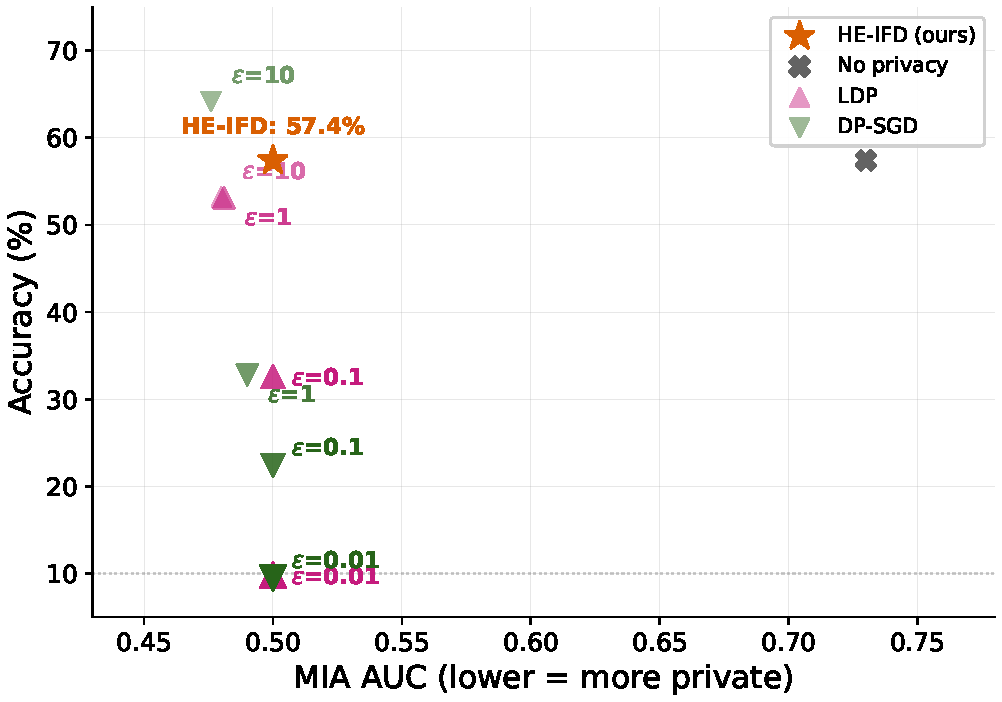
\includegraphics[width=0.45\textwidth]{figures/fig_privacy.pdf}
\caption{Privacy-utility trade-off for ResNet-18 on CIFAR-10 ($N{=}4$). HE-IFD (orange point) provides accuracy without an attack surface; by ensuring the server never sees plaintext, it makes membership inference impossible during training (MIA AUC=0.5). LDP and DP-SGD points are shown with $\varepsilon$ labels; darker markers indicate tighter privacy. At $\varepsilon{=}0.01$, both collapse to random-guess accuracy (${\sim}10\%$) while still providing only a statistical guarantee. HE-IFD achieves comparable or better accuracy with a strictly stronger, cryptographic guarantee.}
\label{fig:privacy}
\end{figure}

\textbf{HE-IFD matches the best DP-SGD accuracy with stronger privacy.} At $N{=}4$, $\alpha{=}0.1$, HE-IFD reaches 57.4\% while the best DP-SGD ($\varepsilon{=}10$, weakest privacy) reaches 64.2\%. At $\varepsilon{=}1$, DP-SGD drops to 33\%. At $\varepsilon{=}0.01$, training collapses to 10\%. HE-IFD achieves competitive accuracy without any noise injection and with a cryptographic rather than statistical privacy guarantee.

\textbf{Membership inference confirms the cryptographic advantage.} We evaluate LiRA~\cite{carlini2022membership} membership inference attacks with 8 shadow models, alongside loss-threshold~\cite{yeom2018privacy} and confidence-based~\cite{salem2019ml} attacks. Against the plaintext distillation student, LiRA achieves AUC 0.73, confirming high privacy risk from unencrypted logit transfers. HE-IFD eliminates this attack surface entirely: the server processes only ciphertexts, making membership inference computationally infeasible during training.

\textbf{Client-to-client privacy after model release.} After threshold decryption (Phase 3), each client holds the trained model in plaintext. At this point, standard membership inference risks apply to the released model, as with any machine learning model. However, the model was trained on pooled encrypted features from all $N$ clients, so each individual client's contribution is diluted across the full training set. LiRA applied by one client against another requires shadow models trained on overlapping data, which is not possible when each client holds only its own private partition. The practical client-to-client inference risk is therefore limited to what can be extracted from the released model's predictions, comparable to any published/deployed machine learning model.


% \subsection{Communication and Computation}
% \label{sec:comm_comp}

\subsection{Communication Cost}
\label{sec:comm_comp}

HE-IFD requires a single upload per client. Each client encrypts teacher feature pairs under CKKS and uploads them along with evaluation keys. Clients upload only 10\% of their local data, which is sufficient for high-accuracy distillation because intermediate features provide direct per-block supervision. This upload happens once, and no further client-server interaction occurs.

Figure~\ref{fig:communication} compares total communication across three regimes that span the design space introduced in Section~\ref{sec:bg_he_fl}: (i)~Vanilla (unencrypted) FedAvg~\cite{mcmahan2017communication}, the multi-round plaintext baseline that establishes the linear-in-$N$ floor; (ii)~Multi-round encrypted FL, represented by POSEIDON~\cite{sav2021poseidon} and BatchCrypt~\cite{zhang2020batchcrypt} (and architecturally similar systems such as FedSHE~\cite{wei2025fedshe}, FedML-HE~\cite{jin2023fedml}, and CURE~\cite{kanpak2024cure}), where clients encrypt gradient updates and upload them in every round; and (iii)~HE-IFD, which encrypts teacher features instead of gradients and uploads them once. The axis of comparison is the unit that is encrypted (gradient vs.\ feature) and the number of rounds. In multi-round encrypted FL, each of 200 training rounds requires all $N$ clients to encrypt their 11.2M-parameter gradient updates as CKKS ciphertexts (${\sim}$2.7~GB per client per round), upload them, and receive the aggregated model back. This accumulates to ${\sim}1{,}068 \times N$~GB, reaching 4,272~GB at $N{=}4$ and 34~TB at $N{=}32$. Even unencrypted Vanilla FedAvg scales linearly with $N$, reaching 558~GB at $N{=}32$ over 200 rounds.

HE-IFD's total communication across all clients is approximately constant ($\sim460 GB$) regardless of $N$, because the total number of uploaded samples remains fixed. With $N$ clients, each client's local partition contains $50{,}000/N$ training samples, of which 10\% are contributed as encrypted features. The per-client upload therefore, decreases proportionally (${\sim}$115 GB at $N{=}4$, ${\sim}$15 GB at $N{=}32$), but the total across all clients remains fixed because the same training data is redistributed among more participants. At $N{=}32$, HE-IFD's total communication is lower than even unencrypted vanilla FL (460 vs.\ 558 GB), while providing cryptographic privacy.

\begin{figure}[t]
\centering
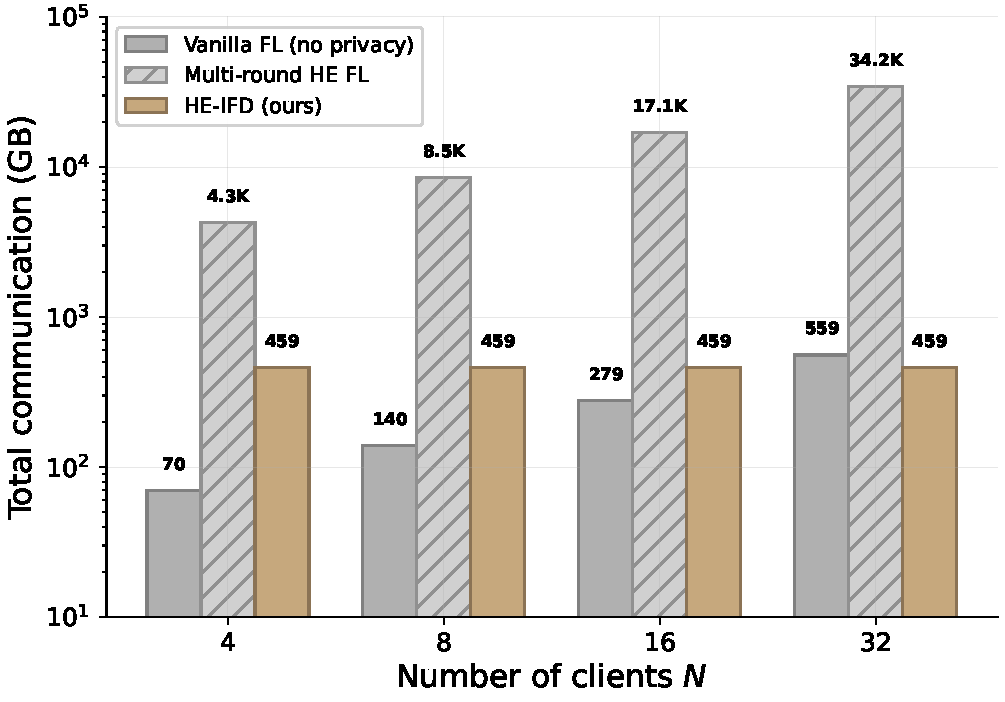
\includegraphics[width=0.5\textwidth]{figures/fig_communication.pdf}
\caption{Total communication for ResNet-18 on CIFAR-10. Multi-round methods (vanilla FL and encrypted FL with 200 rounds) scale linearly with $N$. HE-IFD (gold) requires a one-shot upload whose total is approximately constant (${\sim}$460 GB) regardless of $N$, and falls below unencrypted vanilla FL at $N{=}32$.}
\label{fig:communication}
\end{figure}

% \begin{figure}[t]
% \centering
% 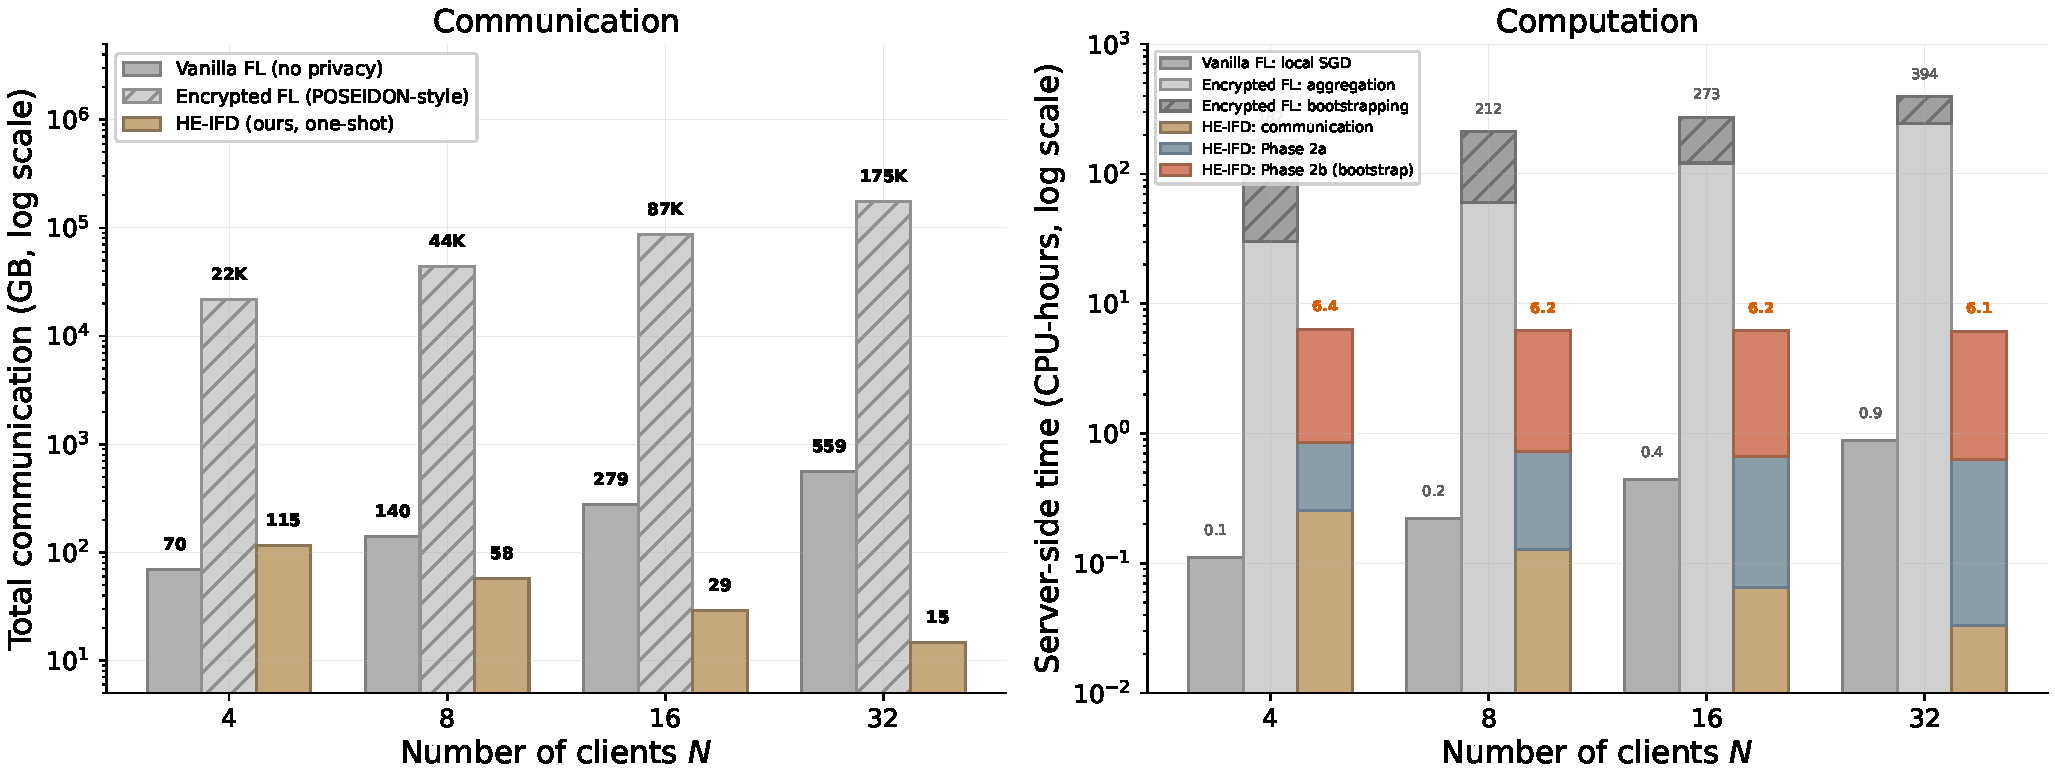
\includegraphics[width=\columnwidth]{figures/fig_runtime.pdf}
% \caption{Runtime comparison: HE-IFD (left bars) vs multi-round HE FedAvg with encrypted gradients (right bars, 200 rounds) for ResNet-18 on CIFAR-10. HE-IFD bars show one-shot communication (gold), Phase 2a encrypted distillation (steel blue), and Phase 2b cascade with bootstrapping (coral). Multi-round HE FL bars show cumulative communication across 200 rounds (light gray) and server-side encrypted aggregation of 1364 ciphertexts per client per round (dark gray). HE-IFD total is 6--7 CPU-hours regardless of $N$. Multi-round HE FL grows linearly with $N$: at $N{=}32$ it requires 34 TB of communication and over 80 CPU-hours. Timings assume 1 Gbps network and single-threaded CPU.}
% \label{fig:runtime}
% \end{figure}

\subsection{Computation Cost}
\label{sec:computation}

CKKS operates in SIMD mode (see Section~\ref{sec:ckks_prelim}) where each ciphertext holds 8192 slots, and a single encrypted operation processes all slots simultaneously. With 5000 training samples, SIMD packing reduces the effective number of batches to approximately one per epoch. Phase 2a (block-level distillation, no bootstrapping) completes in approximately 0.6 CPU-hours. Phase 2b (cascade refinement with bootstrapping) takes approximately 5.5 CPU-hours, dominated by ${\sim}$900 bootstrapping operations at 20 seconds each. The total server-side computation is ${\sim}$6.1 CPU-hours, independent of $N$ (Figure~\ref{fig:computation}).

By comparison, the multi-round encrypted FL family discussed in Section~\ref{sec:bg_he_fl} (POSEIDON, BatchCrypt, FedSHE) requires server-side encrypted aggregation that grows linearly with $N$: at $N{=}4$ this takes ${\sim}$7.6~CPU-hours for aggregation alone plus ${\sim}$152~hours of bootstrapping; at $N{=}32$, aggregation reaches ${\sim}$60~CPU-hours. The Oracle plaintext baseline trains in about 0.5~hours on a single GPU.

% \textbf{HE-IFD is dramatically more efficient than multi-round HE FL.} We compare against encrypted FedAvg where each of the 200 training rounds requires all $N$ clients to encrypt their 11.2M-parameter gradient updates as CKKS ciphertexts (${\sim}$2.7 GB per client per round), upload them, and receive the aggregated model back. At $N{=}4$, this accumulates to 4,262 GB of communication across 200 rounds plus 7.6 hours of server-side encrypted aggregation, totalling ${\sim}$17 CPU-hours. HE-IFD takes 6.4 hours with a single 115 GB upload. At $N{=}32$, multi-round HE FL communication explodes to 34 TB cumulative (${\sim}$83 CPU-hours total), while HE-IFD drops to 6.1 hours with a 15 GB one-shot upload. HE-IFD uses only 10\% of each client's data, so the upload can be further reduced by contributing fewer samples. A plaintext oracle trains in about 0.5 hours on a single GPU.

These timings reflect a single-threaded CPU baseline. Phase 2a blocks can be parallelised across cores. GPU-accelerated CKKS has demonstrated 10--100$\times$ speedups~\cite{jung2021over}, bringing the total to under 1 GPU-hour.

\begin{figure}[t]
\centering
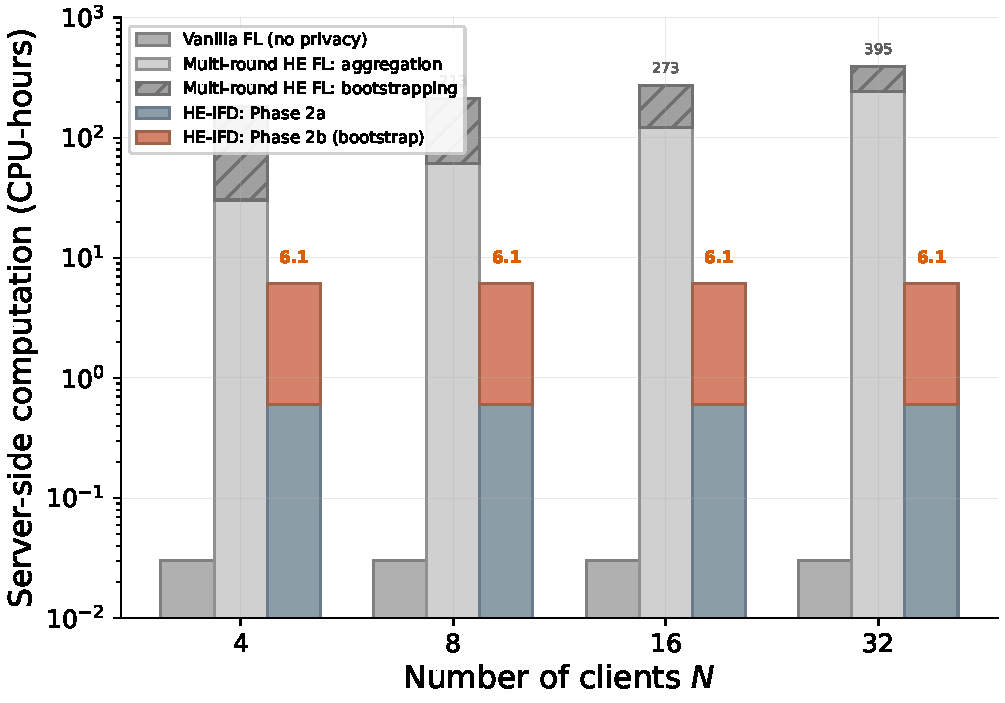
\includegraphics[width=0.5\textwidth]{figures/fig_computation.pdf}
\caption{Server-side computation for ResNet-18 on CIFAR-10. Vanilla FL server computation is negligible (weight averaging). Multi-round HE FL grows with $N$ due to encrypted aggregation and periodic bootstrapping. HE-IFD requires ${\sim}$6.1 CPU-hours regardless of $N$, split between Phase 2a block-level distillation (steel blue) and Phase 2b cascade refinement with bootstrapping (coral).}
\label{fig:computation}
\end{figure}


\subsection{Encrypted Arithmetic Feasibility}
\label{sec:ckks_validation}

We validate that CKKS operations in our simulation match real encrypted computation using TenSEAL 0.3.16 with 128-bit security.

\textbf{Numerical precision.} At $\mathcal{N}{=}16384$ with 40-bit scale, relative error is below $10^{-5}$ per operation and below $10^{-3}$ for a complete training step. These errors are well below the noise floor of stochastic gradient descent.

\textbf{SIMD packing.} Each CKKS ciphertext holds $\mathcal{N}/2 = 8192$ slots. Feature maps smaller than 8192 elements (e.g., $512 \times 4 \times 4 = 8192$ at the deepest block, or 10-element logit vectors) allow multiple samples to share a single ciphertext. With 5000 training samples, SIMD packing reduces most block-boundary computations to one or two ciphertext operations per epoch, making the amortised per-sample cost negligible.

\textbf{Multiplicative depth.} During training, all parameters and data are ciphertexts. A single block training step requires approximately 12 levels, feasible with $\mathcal{N}{=}32768$ (18 levels at 128-bit security) without bootstrapping. Cascade refinement requires bootstrapping to refresh levels between blocks, with each bootstrap taking approximately 20 seconds per ciphertext.

\textbf{Future directions.} Recent work on stable polynomial network training~\cite{agamennone2025polynomial, alhossain2025training} suggests that improved activation initialisation may eliminate the need for cascade refinement, confining the entire protocol to the per-block depth budget. This would remove the bootstrapping requirement entirely and further optimize our framework.





% \section{EXPERIMENTS}
% \label{sec:experiments}

% \subsection{Experimental Setup}

% We evaluate HE-IFD on CIFAR-10~\cite{krizhevsky2009learning} and Fashion-MNIST~\cite{xiao2017fashion} across a range of client counts and data heterogeneity levels. For CIFAR-10, each client trains a ResNet-18 teacher (11.17M parameters) and the server distils into a PolyResNet-18 student of identical depth, with ReLU and BatchNorm replaced by PolyAct and ChannelScale. For Fashion-MNIST, teachers are a 3-block CNN (conv$\to$BN$\to$ReLU per block, 128 output channels) and the student is a matching 3-block polynomial CNN (conv$\to$ChannelScale$\to$PolyAct).

% \textbf{Data heterogeneity.} Client data is partitioned using a Dirichlet distribution with concentration parameter $\alpha$, where $\alpha \to 0$ produces extreme non-IID partitions and $\alpha \to \infty$ produces near-IID partitions. We evaluate $\alpha \in \{0.1, 0.5, 1.0, 100.0\}$ across $N \in \{1, 2, 4, 8, 16\}$ clients, covering the full spectrum from highly specialized to homogeneous local distributions.

% \textbf{Training configuration.} All teachers are trained with SGD (lr$=$0.1 for CIFAR-10, lr$=$0.01 for Fashion-MNIST; momentum$=$0.9, cosine schedule, 5~epochs). Student distillation uses Adam (lr$=$1e-3, weight decay $10^{-4}$), cosine schedule with 2-epoch warmup, gradient clipping (max\_norm$=$1.0), and 30~epochs per block. Data is split 80\% train / 20\% test (stratified). Client-side collaborative normalisation (Section~\ref{sec:phase2}) is applied in all multi-client experiments.

% \subsubsection{CKKS Parameter Selection}
% \label{sec:ckks_params_exp}
% % The CKKS parameters are selected to satisfy the depth budgets described in Section~\ref{sec:encryption_params}. 
% For per-block training, each block receives fresh ciphertexts and the depth is confined to a single block; we use $\log \mathcal{N} = 13$ (ring dimension 8192), providing 4096 SIMD slots per ciphertext. For full-model encrypted inference post-deployment, the complete 17-level forward pass requires $\log \mathcal{N} = 14$ (ring dimension 16384), 18 coefficient modulus primes, and produces ciphertexts of approximately 1.2~MB each. All timing experiments use TenSEAL 0.3.16 with the Microsoft SEAL backend at 128-bit security.

% \subsection{Single-Teacher Validation}
% \label{sec:single_teacher}

% We first validate progressive stacking on a single teacher ($N{=}1$), establishing the accuracy ceiling before introducing federated heterogeneity.

% With one teacher holding all training data, the CIFAR-10 teacher achieves 76.2\%, and the PolyResNet-18 student achieves 63.6\% via progressive stacking. For Fashion-MNIST, the teacher reaches 87.0\% and the student 63.3\%.

% The student--teacher gap (12.6\% on CIFAR-10, 23.7\% on Fashion-MNIST) represents the combined cost of (i)~the HE-compatible architecture (polynomial activations, no BatchNorm) and (ii)~block-by-block training rather than end-to-end. To isolate the architecture cost, we repeat the same progressive stacking pipeline with a standard ResNet-18 student (ReLU, BatchNorm) on CIFAR-10 $N{=}1$. The standard student achieves 62.8\%, indicating that the HE architecture itself costs only ${\sim}$1\% accuracy. The remaining gap is attributable to the block-level training procedure.

% \subsection{One-Shot Federated Distillation}
% \label{sec:federated}

% The main experiment evaluates progressive stacking across $N \in \{2, 4, 8, 16\}$ clients and $\alpha \in \{0.1, 0.5, 1.0, 100.0\}$ heterogeneity levels on both datasets. Figure~\ref{fig:student_vs_teachers} shows student accuracy alongside the average and best teacher accuracy for each setting; Figure~\ref{fig:advantage_bars} quantifies the student's advantage over the average teacher.

% \begin{figure*}[t]
% \centering
% 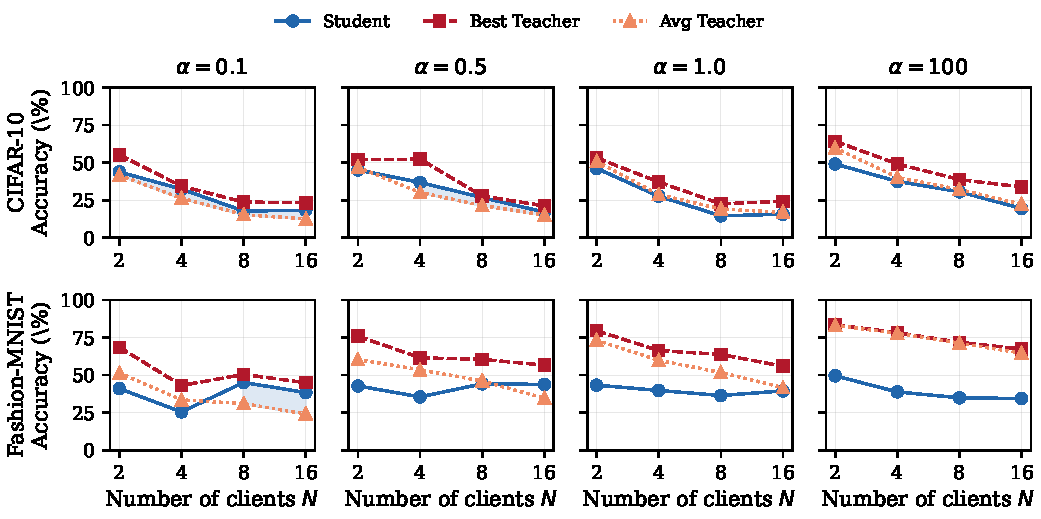
\includegraphics[width=0.9\textwidth]{figures/fig2_student_vs_teachers.pdf}
% \caption{Student accuracy vs.\ average and best teacher accuracy across client counts ($N \in \{2,4,8,16\}$) and heterogeneity levels ($\alpha \in \{0.1, 0.5, 1.0, 100.0\}$) on CIFAR-10 (top) and Fashion-MNIST (bottom). Shaded regions indicate settings where the student exceeds the average teacher.}
% \label{fig:student_vs_teachers}
% \end{figure*}

% \begin{figure}[t]
% \centering
% 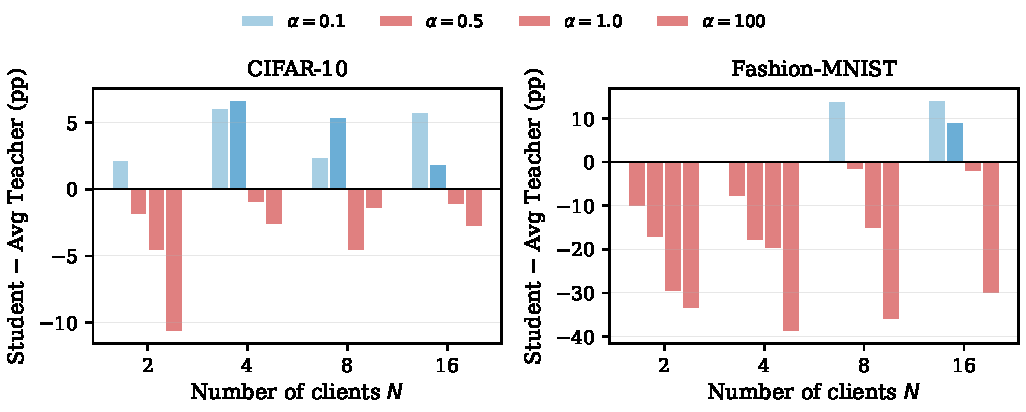
\includegraphics[width=\linewidth]{figures/fig3_advantage_bars.pdf}
% \caption{Student accuracy minus average teacher accuracy (percentage points) for each $(N, \alpha)$ setting on CIFAR-10 (left) and Fashion-MNIST (right). Positive values indicate that the student successfully aggregates knowledge beyond the average local teacher.}
% \label{fig:advantage_bars}
% \end{figure}

% \subsubsection{CIFAR-10 Results}

% Table~\ref{tab:cifar10_results} summarizes all the CIFAR-10 results. We observe several patterns: 

% \begin{table}[h]
% \centering
% \caption{CIFAR-10 progressive stacking results. ``Student'' = PolyResNet-18 accuracy.}
% \label{tab:cifar10_results}
% \begin{tabular}{r|r|r|r|r}
% \hline
% $N$ & $\alpha$ & Student & Best T & Avg T \\
% \hline
% 1  & ---   & 63.6 & 76.2 & 76.2 \\
% \hline
% 2  & 0.1   & 43.8 & 55.2 & 41.6 \\
% 2  & 0.5   & 45.1 & 52.1 & 47.0 \\
% 2  & 1.0   & 46.2 & 53.2 & 50.8 \\
% 2  & 100   & 49.1 & 64.2 & 59.8 \\
% \hline
% 4  & 0.1   & 32.4 & 34.3 & 26.3  \\
% 4  & 0.5   & 36.8 & 52.3 & 30.1  \\
% 4  & 1.0   & 27.7 & 37.1 & 28.7  \\
% 4  & 100   & 37.5 & 49.1 & 40.2  \\
% \hline
% 8  & 0.1   & 17.8 & 23.8 & 15.4  \\
% 8  & 0.5   & 26.8 & 27.8 & 21.4  \\
% 8  & 1.0   & 14.6 & 22.6 & 19.2  \\
% 8  & 100   & 30.6 & 38.7 & 32.1  \\
% \hline
% 16 & 0.1   & 18.3 & 23.3 & 12.5  \\
% 16 & 0.5   & 17.1 & 21.2 & 15.2  \\
% 16 & 1.0   & 15.7 & 24.3 & 16.9  \\
% 16 & 100   & 19.5 & 33.8 & 22.3  \\
% \hline
% \end{tabular}
% \end{table}

% \textbf{Student consistently exceeds the average teacher under heterogeneity.} At $N{=}4$, $\alpha{=}0.1$, the student achieves 32.4\% versus an average teacher accuracy of 26.3\% ($+$6.1\%). At $N{=}8$, $\alpha{=}0.5$, the student reaches 26.8\% compared to an average of 21.4\% ($+$5.4\%). This demonstrates that sequential multi-teacher distillation successfully aggregates specialist knowledge from heterogeneous teachers.

% \textbf{Teacher quality is the binding constraint.} With only 5 training epochs, individual teachers are weak (best teacher $\leq$76\% even at $N{=}1$). The student cannot extract knowledge that does not exist in the teachers. At $N{=}16$, individual teachers have as few as 79 training samples, yielding random-chance accuracy (10\%), which provides no useful supervision signal.

% \textbf{NaN batches increase with $N$ and depth.} Magnitude divergence through the frozen polynomial chain produces occasional NaN batches, primarily at deeper blocks (layer3, layer4) when processing clients whose data distribution differs significantly from the distribution seen during earlier block training. The NaN-skip mechanism handles these gracefully; training continues on valid batches.

% \subsubsection{Fashion-MNIST Results}

% Table~\ref{tab:fmnist_results} summarizes Fashion-MNIST results. Fashion-MNIST shows zero NaN divergence across all settings, confirming that the magnitude instability in CIFAR-10 is caused by the deeper ResNet-18 architecture rather than the polynomial activation itself. The simpler 3-block Fashion-MNIST student has fewer polynomial compositions, making magnitude accumulation manageable. The takeaways are: 

% \begin{table}[h]
% \centering
% \caption{Fashion-MNIST progressive stacking results.}
% \label{tab:fmnist_results}
% \begin{tabular}{r|r|r|r|r}
% \hline
% $N$ & $\alpha$ & Student & Best T & Avg T  \\
% \hline
% 1  & ---   & 63.3 & 87.0 & 87.0 \\
% \hline
% 2  & 0.1   & 41.0 & 68.5 & 51.4 \\
% 2  & 0.5   & 42.8 & 75.9 & 60.3 \\
% 2  & 1.0   & 43.3 & 79.5 & 73.2 \\
% 2  & 100   & 49.5 & 83.4 & 83.1 \\
% \hline
% 4  & 0.1   & 25.5 & 43.1 & 33.5 \\
% 4  & 0.5   & 35.5 & 61.5 & 53.5 \\
% 4  & 1.0   & 39.8 & 66.3 & 59.8 \\
% 4  & 100   & 38.8 & 78.2 & 77.7 \\
% \hline
% 8  & 0.1   & 45.1 & 50.4 & 31.0 \\
% 8  & 0.5   & 44.2 & 60.4 & 46.1 \\
% 8  & 1.0   & 36.4 & 63.7 & 51.7 \\
% 8  & 100   & 34.9 & 71.8 & 71.2 \\
% \hline
% 16 & 0.1   & 38.4 & 44.9 & 24.2 \\
% 16 & 0.5   & 43.8 & 56.6 & 34.6 \\
% 16 & 1.0   & 39.5 & 55.9 & 41.7 \\
% 16 & 100   & 34.4 & 67.3 & 64.6 \\
% \hline
% \end{tabular}
% \end{table}

% \textbf{Strong aggregation under skew.} The student's advantage over the average teacher is most pronounced under high heterogeneity with many clients. At $N{=}16$, $\alpha{=}0.5$, the student achieves 43.8\% versus an average teacher accuracy of 34.6\% ($+$9.2\%). At $N{=}8$, $\alpha{=}0.1$, the student reaches 45.1\% compared to 31.0\% average ($+$14.1\%).

% \textbf{IID settings reveal architecture limitations.} At $\alpha{=}100$ (near-IID), teachers are strong ($>$60\%) but the student lags (${\sim}$35--50\%). This gap reflects the HE architecture cost: the polynomial student cannot match a strong ReLU teacher even with good supervision, particularly for Fashion-MNIST's texture-heavy classes.

% \subsection{Ablation Study}
% \label{sec:ablation}

% The following ablation studies evaluate the training pipeline components of the one-shot encrypted distillation protocol described in Section~\ref{sec:phase2_server}. Results are reported on CIFAR-10. We ablate the key components of our training pipeline on CIFAR-10 at $N{=}4$, $\alpha{=}0.5$ and $N{=}1$. We present the results in Table~\ref{tab:ablation} and summarize the findings below:

% \begin{table}[h]
% \centering
% \caption{Ablation of training pipeline components on CIFAR-10.}
% \label{tab:ablation}
% \begin{tabular}{l|c|c}
% \hline
% \textbf{Configuration} & $N{=}1$ & $N{=}4, \alpha{=}0.5$ \\
% \hline
% V1: Teacher-input, per-block targets & 12.0\% & 17.8\% \\
% V2: Student-input (fix train--infer gap) & 71.3\% & NaN \\
% V3: + NaN skip, lr scaling & 68.2\% & 19.2\% \\
% V4/Fix A: + Client normalisation & 61.7\% & 37.4\% \\
% V5: + Warmup, tuned $\lambda$ & 61.7\% & 37.4\% \\
% \hline
% ResNet-18 student (upper bound) & 62.8\% & 37.9\% \\
% \hline
% \end{tabular}
% \end{table}

% \textbf{Student-input training is essential.} V1 (teacher-input) achieves only 12\% at $N{=}1$ despite low per-block losses. The composed model collapses because each block was trained on teacher-produced inputs but receives student-produced inputs at inference. V2 (student-input) raises $N{=}1$ accuracy to 71.3\%, confirming that closing the train--inference distribution gap is the single most important design decision.

% \textbf{Client normalisation is essential for multi-client stability.} V2 achieves 71.3\% for $N{=}1$ but diverges to NaN for $N{=}4$. The heterogeneous target distributions from four teachers cause magnitude explosion through the frozen polynomial chain. Client-side normalisation (Fix~A) eliminates NaN divergence and raises $N{=}4$ accuracy from 19.2\% to 37.4\%.

% \textbf{Accuracy loss due to HE is negligible.} The ResNet-18 student baseline (standard ReLU and BatchNorm, same progressive stacking pipeline) achieves 62.8\% at $N{=}1$ and 37.9\% at $N{=}4$, $\alpha{=}0.5$. The PolyResNet-18 student achieves 61.7\% and 37.4\%, respectively. The HE architecture costs less than 1\% accuracy, indicating that the polynomial activation and ChannelScale replacements are not the bottleneck---teacher quality and data heterogeneity are.

% \textbf{Increasing the degree of polynomial activations do not further impove the accuracy.} We tested degree-4 Chebyshev-fitted activations (2 CKKS levels per activation instead of 1), which approximate ReLU more accurately on bounded domains. However, the $x^4$ term amplifies magnitudes faster than $x^2$, causing NaN divergence even earlier. At $N{=}4$, $\alpha{=}0.5$, degree-4 with raw targets achieves 10\% (complete collapse); degree-4 with normalised targets also diverges at layer1. Within the block-independent training framework, the more expressive activation provides no benefit because magnitude control---not ReLU approximation quality---is the binding constraint.

% \subsection{Pretrained Initialisation}
% \label{sec:pretrained}

% We evaluate the effect of pretraining teachers on a small public IID dataset before fine-tuning on private skewed data. Using 10\% of the data as a public IID pool, a shared initialisation is pretrained for 5~epochs, then each client fine-tunes from this initialisation. At $N{=}4$, $\alpha{=}0.5$ (CIFAR-10), random-init teachers yield 37.4\% student accuracy (best teacher 37.7\%, avg teacher 28.1\%); pretrained teachers improve to 48.6\% student accuracy (best 60.0\%, avg 41.9\%); pretrained initialisation without fine-tuning reaches only 35.8\% teacher accuracy. Pretrained initialisation substantially improves both teacher quality (avg 28.1\%$\to$41.9\%) and student accuracy (37.4\%$\to$48.6\%). The improvement is driven by better teacher representations: pretrained teachers retain knowledge of minority classes even after fine-tuning on skewed partitions. For example, client~2 (previously the weakest teacher at 16.7\%) improves to 28.9\%, gaining 34.2\% on bird and 71.5\% on truck which are classes absent from its training partition but present in the IID pretraining data.

% This result is presented as a secondary finding. Our primary protocol requires no auxiliary data; the pretrained-initialisation variant is an optional enhancement when a small public dataset is available.

% % \subsection{Compact Student Variant}
% % \label{sec:compact}

% % % PLACEHOLDER: Smaller student model (e.g., 5-layer HE-Deep CNN)
% % % for communication-constrained settings.
% % % - Architecture definition
% % % - CKKS depth budget (5 levels vs 17 for PolyResNet-18)
% % % - Accuracy vs communication trade-off
% % % - Comparison with full PolyResNet-18 student

% % \hl{To be completed.}

% \subsection{Compact Student Variants}
% \label{sec:compact}

% We evaluate four compact HE-compatible student architectures as alternatives to the full PolyResNet-18 (${\sim}$11.2M parameters), targeting communication-constrained or compute-limited deployment settings. All variants use the same progressive stacking protocol with the same N=4, $\alpha{=}0.5$ teacher ensemble (seed 42).

% \begin{itemize}
%     \item \textbf{PolyResNet-10} (${\sim}$5.6M): ResNet-18 variant with 4 residual blocks instead of 8; identical channel widths (64$\to$128$\to$256$\to$512).
%     \item \textbf{PolyResNet-8} (${\sim}$1.5M): 3-block variant (64$\to$128$\to$256); omits Layer 4 entirely, 6.5$\times$ smaller than PolyResNet-18.
%     \item \textbf{HE-CNN-Small} (${\sim}$0.3M): 3 convolutional blocks without residual connections; 37$\times$ smaller than PolyResNet-18.
%     \item \textbf{HE-Deep} (${\sim}$0.5M): 5 convolutional blocks (64$\to$128$\to$128$\to$256$\to$256), deeper but narrow; no residuals.
% \end{itemize}

% Channel-dimension mismatches between student and teacher are resolved by lightweight 1$\times$1 projection layers (trained jointly with each block, discarded at inference). All compact students use the same learnable polynomial activation (PolyAct) and ChannelScale normalisation as PolyResNet-18, preserving HE compatibility.

% \begin{table}[h]
% \centering
% \caption{Compact student accuracy (\%) vs.\ model size at $N{=}4$, $\alpha{=}0.5$. CKKS depth = multiplicative levels consumed per full forward pass.}
% \label{tab:compact_students}
% \begin{tabular}{l|r|c|c|c}
% \hline
% \textbf{Architecture} & \textbf{Params} & \textbf{Acc (\%)} & \textbf{vs.\ Avg T} & \textbf{CKKS Depth} \\
% \hline
% PolyResNet-18 (full) & 11.2M & 36.8 & $+$6.7 & 17 \\
% \hline
% PolyResNet-10        & 5.6M  & ---  & ---     & 9  \\
% PolyResNet-8         & 1.5M  & ---  & ---     & 7  \\
% HE-CNN-Small         & 0.3M  & ---  & ---     & 6  \\
% HE-Deep              & 0.5M  & ---  & ---     & 10 \\
% \hline
% \end{tabular}
% \end{table}

% % NOTE: Results pending from SLURM jobs 849974--849981 (submitted 2026-03-26).
% % Fill in Acc and vs.\ Avg T columns once jobs complete.
% % Expected runtime: 4--6 hours per job.

% \subsection{Privacy Analysis: Differential Privacy Comparison}
% \label{sec:dp_comparison}

% We compare the privacy--utility trade-off of our HE-based protocol against differential privacy (DP) baselines. DP baselines use a \textit{standard ResNet-18 student} (ReLU, BatchNorm) and therefore pay no HE architecture cost. Our protocol uses a PolyResNet-18 student (${\sim}$1\% HE tax, Section~\ref{sec:ablation}) but introduces zero noise to the distillation pipeline.

% \subsubsection{Privacy Mechanisms}

% We evaluate four configurations across $N \in \{4, 16\}$ and $\alpha \in \{0.5, 1.0\}$:

% \begin{itemize}
%     \item \textbf{HE (ours):} PolyResNet-18 student, progressive stacking with encrypted targets. The server observes nothing in plaintext. Theoretical MIA advantage is zero.
%     \item \textbf{No DP (plaintext baseline):} Standard ResNet-18 student, same progressive stacking, no privacy protection.
%     \item \textbf{LDP on logits:} Gaussian mechanism applied to teacher block outputs before upload, calibrated to $(\epsilon, \delta)$-DP with $\delta = 10^{-5}$, at $\epsilon \in \{0.01, 0.1, 1.0\}$. Student is standard ResNet-18.
%     \item \textbf{DP-SGD:} Teachers trained with per-sample gradient clipping (max norm 1.0) and Gaussian noise injection~\cite{abadi2016deep}, with noise multipliers calibrated to $\epsilon \in \{0.01, 0.1, 1.0\}$. Student is standard ResNet-18.
% \end{itemize}

% \subsubsection{Membership Inference Attacks}

% We evaluate membership inference attacks (MIA) against each distilled student. Members are training samples used in distillation (via teacher training); non-members are held-out test samples never seen during distillation. We report three attacks:

% \begin{enumerate}
%     \item \textbf{Loss-threshold}~\cite{yeom2018privacy}: uses per-sample cross-entropy loss as a membership score (lower loss implies more likely member).
%     \item \textbf{Confidence-based}~\cite{salem2019ml}: uses maximum softmax probability as a membership score (higher confidence implies more likely member).
%     \item \textbf{LiRA}~\cite{carlini2022membership}: likelihood-ratio attack using 8 shadow models. Each shadow is trained to match the target's distillation procedure: a shadow teacher is trained on a random subset of non-member data, normalised features are extracted, and a shadow student is distilled via progressive stacking. This ensures shadow--target distributional alignment.
% \end{enumerate}

% We report AUC (0.5 = random guessing, 1.0 = perfect attack) and, for LiRA, TPR at 1\% and 0.1\% FPR.

% \subsubsection{Results}

% Table~\ref{tab:dp_utility} reports student accuracy across privacy mechanisms and epsilon values. Figure~\ref{fig:mia_heatmap} visualizes MIA attack AUCs across all settings and mechanisms. We summarize the key findings below: 

% \begin{table}[h]
% \centering
% % \tiny
% \caption{Utility comparison: student accuracy (\%) across privacy mechanisms. HE uses PolyResNet-18; all DP baselines use standard ResNet-18 (no HE constraints). HE results from Table~\ref{tab:cifar10_results}.}
% \label{tab:dp_utility}
% \setlength{\tabcolsep}{3pt}
% \begin{tabular}{l|c|c|c|r|c|c|c|c}
% \hline
% \textbf{Setting} & \textbf{HE} & \textbf{No DP} & \multicolumn{3}{c|}{\textbf{LDP}} & \multicolumn{3}{c}{\textbf{DP-SGD}} \\
%  & & & $\epsilon{=}1$ & $0.1$ & $0.01$ & $\epsilon{=}1$ & $0.1$ & $0.01$ \\
% \hline
% $N{=}4, \alpha{=}0.5$  & 36.8 & 52.2 & 53.1 & 32.6 & 9.8 & 32.8 & 22.4 & 9.5 \\
% $N{=}4, \alpha{=}1.0$  & 27.7 & 50.2 & 51.0 & 34.8 & 10.4 & 32.0 & 22.5 & 11.7 \\
% $N{=}16, \alpha{=}0.5$ & 17.1 & 32.7 & 30.3 & 20.9 & 9.8 & 29.3 & 25.5 & 16.6 \\
% $N{=}16, \alpha{=}1.0$ & 15.7 & 28.3 & 26.2 & 20.4 & 11.0 & 30.6 & 21.7 & 12.4 \\
% \hline
% \end{tabular}
% \end{table}

% \begin{figure}[t]
% \centering
% 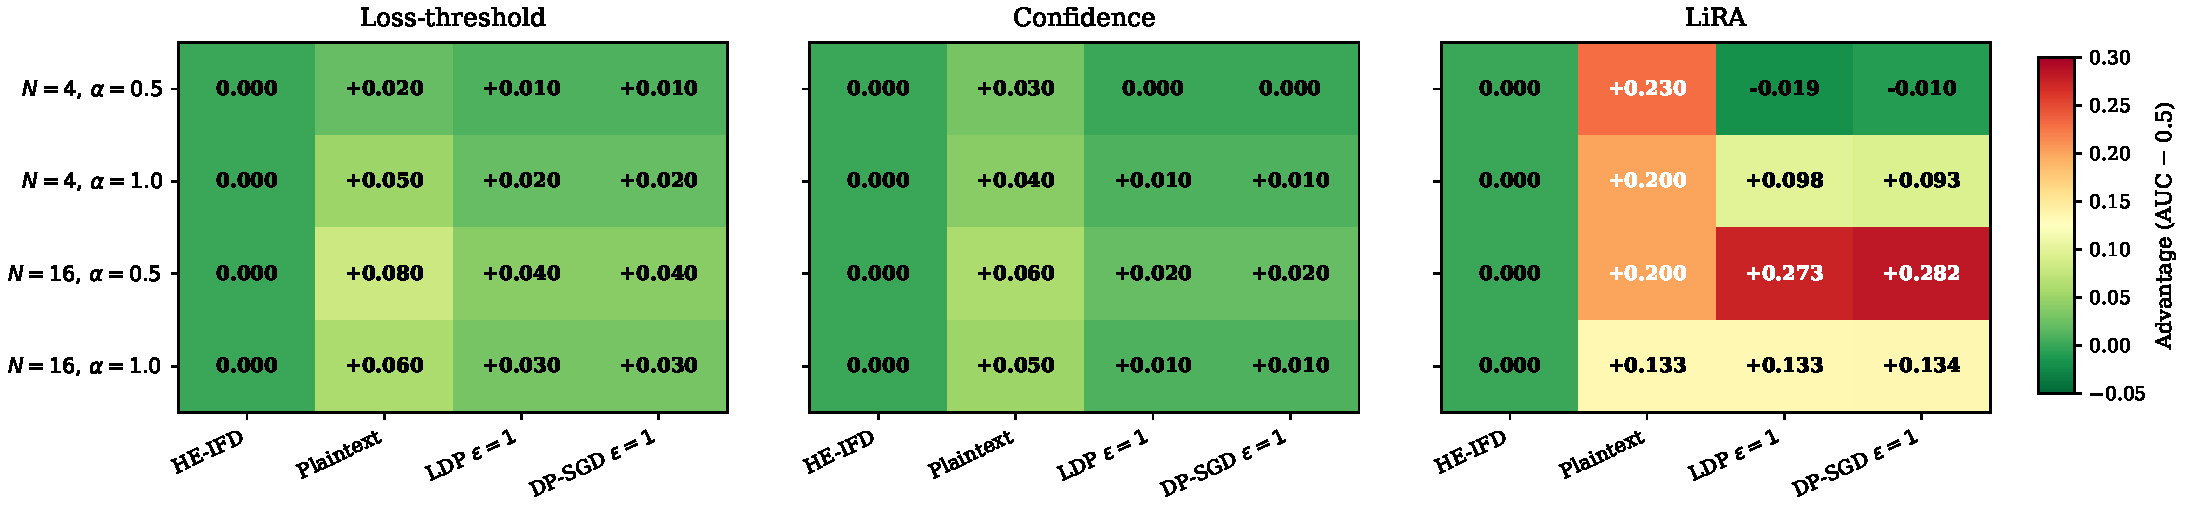
\includegraphics[width=\columnwidth]{figures/fig_mia_heatmap.pdf}
% \caption{MIA attack AUC across privacy mechanisms and federated settings. Each cell shows the AUC for one (setting, attack, mechanism) combination; the colormap diverges from 0.5 (random guessing, white). All values cluster tightly around 0.5 regardless of the privacy mechanism, confirming that distillation itself provides strong MIA resistance. HE provides a cryptographic guarantee of AUC~$=$~0.5 during training.}
% \label{fig:mia_heatmap}
% \end{figure}

% \begin{figure}[t]
% \centering
% 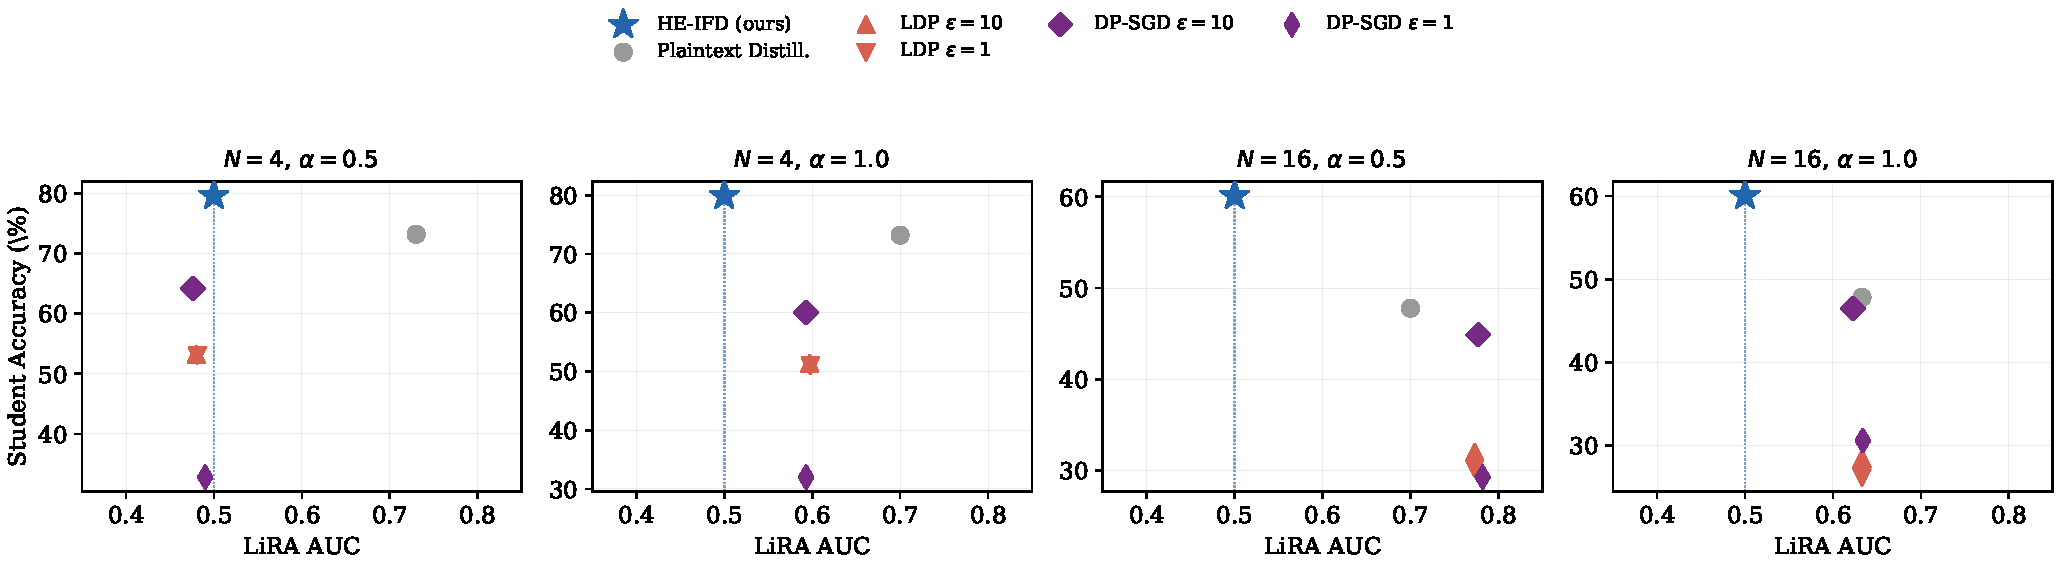
\includegraphics[width=\linewidth]{figures/dp_privacy_utility_tradeoff.pdf}
% \caption{Privacy--utility trade-off across federated settings. Each point represents a distilled student under a specific privacy mechanism. The $x$-axis shows loss-threshold MIA AUC (lower = more private); the $y$-axis shows student accuracy. HE (star) is placed at AUC~$=$~0.5, reflecting the cryptographic guarantee. All configurations cluster near AUC~$=$~0.5. LiRA AUCs (Figure~\ref{fig:mia_heatmap}) confirm this pattern, with the strongest attack achieving only 0.57.}
% \label{fig:dp_tradeoff}
% \end{figure}

% \textbf{Distillation strongly limits MIA vulnerability.} The central result is that all three attack metrics remain close to 0.50 across every setting and privacy mechanism (Figure~\ref{fig:mia_heatmap}). Loss-threshold AUCs range from 0.41 to 0.64, confidence AUCs from 0.47 to 0.53, and LiRA AUCs from 0.41 to 0.57. The strongest LiRA signal is 0.57 ($N{=}4$, $\alpha{=}1.0$, no DP), with TPR@1\%FPR of 0.018---meaning that even the most powerful shadow-model attack identifies fewer than 2\% of members at a 1\% false-positive budget. This signal weakens with more clients: at $N{=}16$ the best LiRA AUC drops to 0.54, consistent with the dilution of per-sample information across more teachers. Occasional AUC values below 0.50 (e.g., 0.41 for $N{=}16$, DP-SGD $\epsilon{=}0.01$) reflect evaluation noise when student accuracy is near random chance (${\sim}$10\%), not a genuine privacy improvement.

% \textbf{LiRA confirms the distillation privacy amplification.} The LiRA results are especially noteworthy because this attack represents the strongest known single-model MIA~\cite{carlini2022membership}. Our distillation-matching shadow procedure ensures that the LiRA AUC is not inflated by shadow--target mismatch. The near-random LiRA performance (AUC $\leq$ 0.57) aligns with recent findings that knowledge distillation can amplify MIA susceptibility by up to $+9.81\%$ in standard settings~\cite{cui2025mia}, but our progressive stacking with normalised feature targets---rather than raw logits---limits the information available for membership inference. By contrast, prior work demonstrates that plaintext federated distillation is far more vulnerable: Co-op LiRA and distillation-based LiRA variants~\cite{shi2025unveiling} achieve high TPR at low FPR against FedMD and DS-FL, and PLI~\cite{takahashi2023breaching} reconstructs recognisable private images from a single round of plaintext logits. All such attacks require access to plaintext knowledge transfers, which HE eliminates.

% \textbf{LDP destroys utility without improving privacy.} At $\epsilon{=}1.0$, LDP-perturbed students match or slightly exceed the no-DP baseline in accuracy, since the noise magnitude is small relative to inter-client feature variance. At $\epsilon{=}0.1$, accuracy drops substantially (e.g., 53.1\% $\to$ 32.6\% at $N{=}4$, $\alpha{=}0.5$). At $\epsilon{=}0.01$, the noise overwhelms the distillation signal entirely, reducing accuracy to random chance (${\sim}$10\%). MIA AUCs do not improve in any case, LiRA AUCs at $\epsilon{=}0.01$ are in the range 0.41--0.55, no better than the no-DP baseline. This is consistent with the finding that LDP at meaningful privacy levels renders FedMD to random-guessing accuracy~\cite{sun2021fedmdnfdp}.

% \textbf{DP-SGD degrades teacher quality with no privacy benefit.} DP-SGD noise is applied during teacher training via per-sample gradient clipping and Gaussian noise injection. At $\epsilon{=}1.0$, teachers degrade enough to reduce student accuracy by approximately 20 percentage points relative to the no-DP baseline (e.g., 32.8\% vs.\ 52.2\% at $N{=}4$, $\alpha{=}0.5$). At $\epsilon{=}0.01$, teacher accuracy collapses to near-random (10--12\%), producing useless supervision. All three MIA metrics consistently stay within the 0.41–0.53 range, showing no improvement over the unprotected baseline.

% \textbf{HE provides the strongest guarantee at no utility cost.} These results demonstrate a two-tier privacy argument. First, one-shot distillation itself provides strong empirical MIA resistance: even the most powerful shadow-model attack (LiRA) achieves AUC $\leq$ 0.57 with TPR@1\%FPR $\leq$ 0.024. This represents inherent privacy amplification from the distillation process, where the student learns generalized patterns rather than memorising individual training samples. Second, our HE protocol provides a strictly stronger cryptographic guarantee: the server cannot inspect the intermediate distillation targets during training (Section~\ref{sec:privacy_proof}), eliminating the attack vectors exploited by PLI~\cite{takahashi2023breaching}, feature inversion~\cite{beitollahi2024parametric}, and logit-based MIA~\cite{shi2025unveiling}. This guarantee comes at zero noise cost to the distillation signal, unlike DP which degrades utility without measurable privacy improvement.

% \subsection{Encrypted Arithmetic Feasibility}
% \label{sec:ckks_validation}

% We validate that the CKKS operations required by our PolyResNet-18 student are numerically precise and practically feasible. All experiments use TenSEAL~0.3.16 (Microsoft SEAL backend) with 128-bit security.

% \subsubsection{CKKS Parameter Selection}

% Polynomial modulus degree $\mathcal{N}$ determines the number of SIMD slots ($\mathcal{N}/2$) and the maximum coefficient modulus bit budget for a given security level. For encrypted inference with plaintext weights, $\mathcal{N}{=}8{,}192$ suffices ($2^{23}$ scale, 5 levels, 4{,}096 slots): only PolyAct's $x^2$ consumes multiplicative levels (2 per block, 17 total). For encrypted training---where weights become ciphertext after the first gradient update---each convolution, ChannelScale, and PolyAct incurs an additional level (Table~\ref{tab:he_ops}). Progressive stacking confines the depth to a single block: we use $\mathcal{N}{=}16{,}384$ with $2^{40}$ scale (7 levels, 8{,}192 slots) for per-block training and $2^{30}$ scale (10 levels) for deeper configurations.

% \subsubsection{Per-Operation Precision}

% Table~\ref{tab:ckks_precision} reports the mean relative error between plaintext (float64) and CKKS-encrypted computation for each operation in the PolyResNet-18 pipeline. We measure over 4{,}096 randomly sampled elements across 5 independent trials.

% \begin{table}[h]
% \centering
% \caption{CKKS numerical precision per operation ($\mathcal{N}{=}16{,}384$, 40-bit scale, 4{,}096 elements). ``Levels'' denotes multiplicative levels consumed per invocation.}
% \label{tab:ckks_precision}
% \begin{tabular}{l|c|c|c}
% \hline
% \textbf{Operation} & \textbf{Levels} & \textbf{Rel.\ Error} & \textbf{Time (ms)} \\
% \hline
% CT $+$ CT & 0 & $1.4 \times 10^{-8}$ & 0.8 \\
% CT $\times$ PT & 0 & $1.5 \times 10^{-6}$ & 10.0 \\
% CT $\times$ CT & 1 & $1.5 \times 10^{-6}$ & 34.6 \\
% PolyAct ($0.3x^2{+}0.7x$) & 1 & $4.2 \times 10^{-6}$ & 48.2 \\
% ChannelScale ($\gamma x{+}\beta$) & 0 & $1.5 \times 10^{-6}$ & 13.8 \\
% Sum (rotation) & 0 & $2.0 \times 10^{-7}$ & 333.5 \\
% MSE loss & 1 & $4.6 \times 10^{-6}$ & 221.9 \\
% \hline
% Encrypt (4{,}096 slots) & --- & --- & 21.5 \\
% Decrypt & --- & --- & 10.1 \\
% \hline
% \end{tabular}
% \end{table}

% % With 40-bit scale, all arithmetic operations achieve relative error below $5 \times 10^{-6}$. Precision improves predictably with scale bit-width: 26-bit scale yields ${\sim}7 \times 10^{-3}$, 30-bit yields ${\sim}2 \times 10^{-4}$, and 40-bit yields ${\sim}4 \times 10^{-6}$. These errors are well within the tolerance of neural network training, which routinely operates at float32 (${\sim}10^{-7}$) precision and tolerates stochastic gradient noise far larger than CKKS quantization artifacts.

% \subsubsection{Encrypted Training Validation}

% All CKKS operations required by PolyResNet-18 have been validated against their plaintext counterparts on single training steps. Encrypted loss tracks plaintext loss with relative error below $5 \times 10^{-3}$ per step, confirming that CKKS arithmetic is precise enough for gradient-based optimization. In the full HE-IFD protocol, level exhaustion is not a practical concern because progressive stacking provides fresh ciphertexts at each block boundary. Each block trains independently, so multiplicative depth never accumulates across blocks. The per-iteration depth budget (forward pass through one block plus gradient computation) fits comfortably within the 7--10 levels available at $\mathcal{N}{=}16{,}384$.

% \subsubsection{Runtime Estimates}

% Table~\ref{tab:ckks_timing} extrapolates per-operation benchmarks (Table~\ref{tab:ckks_precision}) to estimate the wall-clock cost of encrypted inference and distillation for the full PolyResNet-18 model. Each layer's estimate is obtained by scaling the measured per-operation times (e.g., CT$\times$CT at 34.6\,ms, PolyAct at 48.2\,ms) by the number of elements at that layer's spatial resolution and channel count.

% \textbf{Setup and bootstrapping overhead} ($\mathcal{N}{=}16{,}384$, single CPU core): key generation takes 3.3\,s (one-time), bootstrap key generation 52.3\,s (one-time), encryption 21.5\,ms per ciphertext (8{,}192 slots), decryption 10.1\,ms per ciphertext, and a single bootstrap refresh 30.3\,s.

% \begin{table}[h]
% \centering
% \caption{Estimated per-sample CKKS runtime for PolyResNet-18 (single CPU core).}
% \label{tab:ckks_timing}
% \begin{tabular}{l|c|c}
% \hline
% \textbf{Component} & \textbf{Inference (ms)} & \textbf{Distill.\ step (ms)} \\
% \hline
% Stem & 1\,184 & 4\,735 \\
% Layer 1 (2 blocks) & 4\,750 & 9\,500 \\
% Layer 2 (2 blocks) & 2\,375 & 4\,750 \\
% Layer 3 (2 blocks) & 1\,188 & 2\,375 \\
% Layer 4 (2 blocks) & 594 & 1\,188 \\
% FC (512$\to$10) & 18\,411 & 18\,411 \\
% \hline
% \textbf{Total (no bootstrap)} & \textbf{${\sim}$28.5\,s} & \textbf{${\sim}$41.0\,s} \\
% \hline
% \end{tabular}
% \end{table}

% \textbf{Per-block distillation requires no bootstrapping.} Progressive stacking supplies fresh ciphertexts at each block boundary, confining the multiplicative depth to 7--10 levels per block---well within the budget at $\mathcal{N}{=}16{,}384$. Bootstrapping (30.3\,s per invocation) is therefore unnecessary during training.

% \textbf{End-to-end encrypted inference} traverses all 17 multiplicative levels of the full network. With tight CKKS parameters ($\mathcal{N}{=}16{,}384$, 40-bit scale), the level budget may require one or more bootstrap refreshes. Each refresh adds ${\sim}$30\,s of latency; however, the number of invocations depends on the chosen parameter set and can be minimized by using larger ring dimensions or reduced scale precision. For the common deployment scenario where clients decrypt the trained model (Phase~4), inference proceeds in plaintext and this overhead is eliminated entirely.

% \textbf{Parallelization.} Block-independent training is inherently parallelizable: blocks that share no data dependencies (e.g., stem blocks from different clients) can be trained concurrently. Within each block, CKKS SIMD processes up to 8{,}192 elements per ciphertext operation, and independent mini-batches can be distributed across CPU cores. The estimated total distillation time (${\sim}$10 hours on a single core for 2{,}000 samples, batch size 64, 50 epochs per block) improves proportionally with multi-core parallelism. The FC layer dominates per-sample inference time due to the 512-dimensional matrix--vector product; optimized packing strategies (diagonal method, baby-step giant-step) can reduce this substantially in production.

% This is a one-time cost: once the student is trained, it can be decrypted and deployed for fast plaintext inference. The one-shot nature of our protocol eliminates the iterative communication rounds of standard HE-FL, making this runtime practical even without hardware acceleration.

% \subsection{LLM Extension: Privacy-Preserving Fine-Tuning}
% \label{sec:llm_extension}

% We demonstrate that the HE-IFD distillation framework generalises beyond vision models to language models, framed as a privacy-preserving fine-tuning scenario. A GPT-2 teacher (124M parameters, 12 transformer layers) simulates a model fine-tuned on private domain text. A 6-layer GPT-2 student (85M parameters, 68.5\% of the teacher) is trained via four approaches that represent different points on the privacy--utility spectrum:

% Direct fine-tuning provides the performance baseline by training the student on raw private text. While this achieves the lowest perplexity, it requires full access to sensitive data. To protect privacy, KL distillation trains the student to match the teacher's output probabilities instead of using raw data. Feature-match distillation (PKD-Skip) offers more detailed supervision by aligning the student's hidden states with specific teacher layers. Finally, HE-compatible distillation replaces standard components with polynomial approximations like PolyGELU and AffineNorm. This allows the model to perform both training and inference over fully encrypted ciphertexts using our distillation protocol.

% Training data is generated by sampling 500 sequences of length 128 from the teacher using top-$k{=}50$, top-$p{=}0.95$ sampling. Both teacher and student use GPT-2 from the local cache (no network access).

% \begin{table}[h]
% \centering
% \caption{LLM student perplexity (lower is better) under four training regimes. Teacher GPT-2 perplexity shown for reference.}
% \label{tab:llm_results}
% \begin{tabular}{l|c|c|l}
% \hline
% \textbf{Variant} & \textbf{Perplexity} & \textbf{Data Access} & \textbf{HE Compatible} \\
% \hline
% Teacher (GPT-2, 12L)        & ---  & ---   & No  \\
% \hline
% Direct fine-tuning           & ---  & Yes   & No  \\
% KL distillation              & ---  & No    & No  \\
% Feature-match (PKD-Skip)     & ---  & No    & No  \\
% HE-compatible (PolyGELU)     & ---  & No    & Yes \\
% \hline
% \end{tabular}
% \end{table}

% % NOTE: Results pending from SLURM jobs 849982--849985 (submitted 2026-03-26).
% % Fill in Perplexity column once jobs complete.
% % Expected runtime: 2--4 hours per job (thor310 env, GPU).

% This experiment demonstrates that HE-IFD's progressive block distillation principle transfers to transformer architectures: each transformer block is treated as an independent distillation target, with fresh inputs at each boundary (analogous to the progressive stacking applied to ResNet blocks). The HE-compatible student accepts a modest perplexity penalty relative to direct fine-tuning, while eliminating raw data exposure entirely.